% example with several commonly used tex constructs
\section{Section}

Example citation \cite{CBM-stat-rep}. Entry must be in
dabc-bibitems.tex.\\ % new line

Example figure
\begin{figure}[htb]
\centering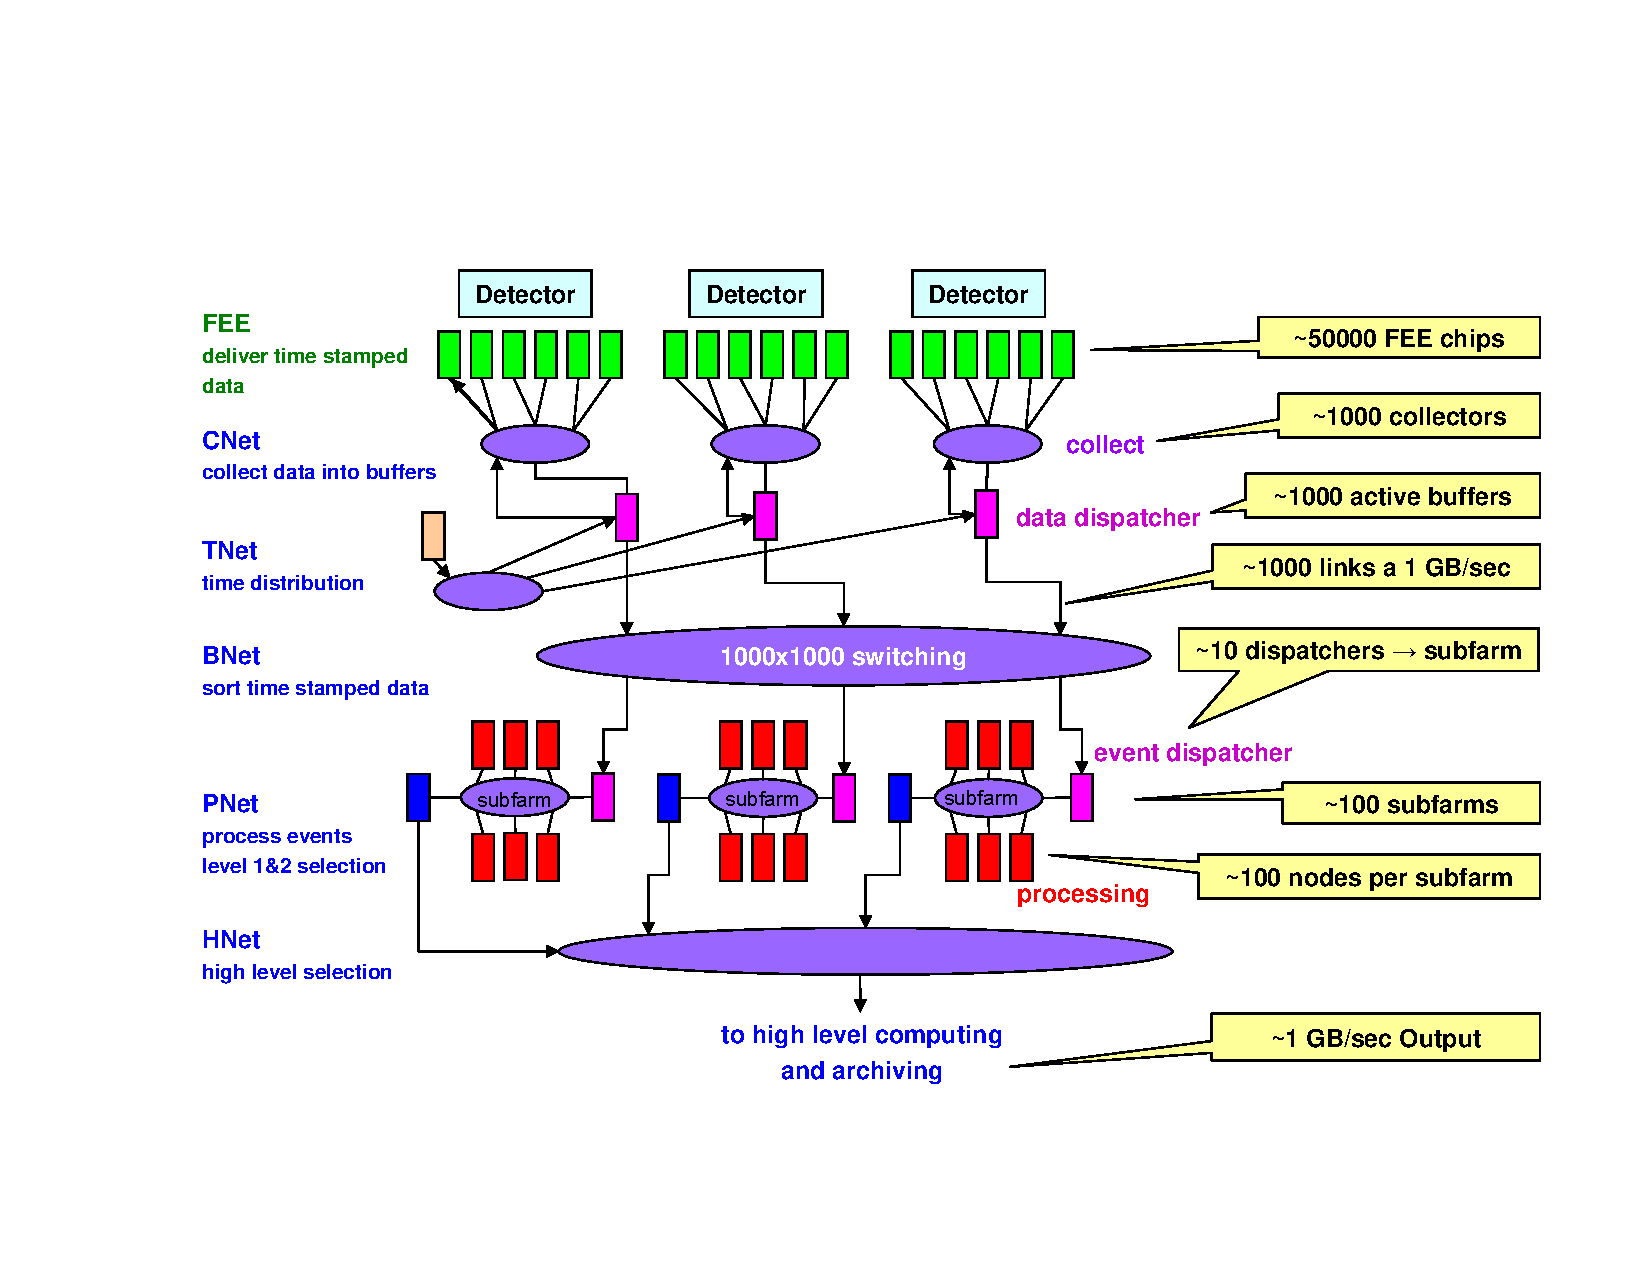
\includegraphics[angle=-90,width=.8\textwidth]{dabcf-daq-all} % pdf file
\caption{CBM overall data processing architecture}
\label{fig:XXX-fig} % give it a name for references
\end{figure}

\index{DABC!mission} % entry in index

Reference to Fig.~\ref{fig:XXX-fig}.
\clearpage % new page

\section{Next section}
\index{DABC!mission} % entry in index

% define a marker to be referenced from outside:
\hyperdef{XXX}{name}{[Marker:XXX:name]}\\
% Reference to external paper having a \hyperdef{sw}{data}
See also \hyperref{http://dabc.gsi.de/doc/manuals/main-software.pdf}{sw}{data}{Software paper}.\\
See also \hyperref{http://dabc.gsi.de/doc/manuals/main-intro.pdf}{in}{mission}{Introduction paper}.

\subsection{Subsection}
\index{DABC!technology} % entry in index

Example of a compact list with bullets
\bbul
\item FEE: self-triggered, data push, conditional RoI based readout
\item CNet: combined data, time, control, and RoI traffic
\ebul

Another compact list with circles
\bcir
\item Hardware
\item Firmware
\ecir

Another compact list with triangle
\btri
\item Hardware
\item Firmware
\etri

Another compact list with squares
\bbox
\item Hardware
\item Firmware
\ebox

\subsubsection{Subsubsection}

Example of compact description list
\bdes
\item[Hardware] There are mainly three boards with different tasks but similar architecture.
\item[Data formats] The data and time stamp formats must be defined early because they are
interpreted at many occasions. A change would have big impact.
\edes

Example of compact numerated list
\bnum
\item compressed
\item coded geographical address
\enum

Example of table
\begin{table}[h]
\begin{tabular}{|p{2.0cm}|p{2.0cm}|p{3.0cm}|p{1.6cm}|p{5.0cm}|}      \hline
Document   & Date        & Editor       & Revision & Comment      \\ \hline
DAS-XXX-06 & 2006 Mar 13 & Hans G.Essel & 0.9      & First scetch \\ \hline
\end{tabular}
\caption{Example of table.}
\label{XXX-table}
\end{table}

When we have a \class{MyNewClass} it might have some \func{Functions} and some \member{Members}.
It also might have some \keyw{Constants} and \decl{Declarations}.
Fixed terms should be in \verba{Typewriter}. Text to be highlighted: \strong{Note!}.
DIM parameter and commands as \param{DataRate} and \comm{setBufferSize}
